\section{Theorie}
\label{sec:Theorie}
Ein Laser (light amplification by stimulated emission of radiation) ist eine monochromatische Lichtquelle mit hoher Kohärenz und Intensität.


\subsection{Funktionsprinzip eines Lasers}
Ein Laser besteht aus drei grundlegenden Komponenten: einem aktiven Medium, einem Resonator und einer Pumpquelle. In dem aktiven Medium werden durch die Pumpquelle Atome angeregt. Diese emittieren bei der Rückkehr auf ein niedrigeres
Energieniveau ein Photon mit der Energie des Übergangs. Diese Emissionen können durch Stimulation oder spontan auftreten.\\
Ein spontanes Auftreten ist dabei der Zerfall eines instabilen Energiezustands. Dies führt zu einer Emission des Photons in eine zufällige Raumrichtung. Die so erzeugten Photonen haben zwar, wenn sie aus demselben Energieniveau-Übergang,
dieselbe Wellenlänge wie es für den Laser erwartet wird, aber sie können nur verstärkt werden, wenn sie zufällig in die richtige Raumrichtung emittiert werden. Damit sind die meisten für den Laserstrahl nicht nutzbar. Der kleine Teil der
Photonen, die sich entlang der Resonatorachse bewegen, können den Laserprozess starten.\\
Die angeregte Emission dagegen wird durch ein eintreffendes Photon, der Energie, wie die Energiedifferenz der Energieniveaus aus der das Laserlicht entstehen soll, stimuliert. Die hierzu ursprünglich nötigen Photonen werden durch
die, von der Pumpquelle angetreten, Atomen durch spontane Emission erzeugt. Diese bewegen sich gerichtet entlang der Achse des Resonators. Auf dem Weg durch das aktive Medium treffen diese Photonen auf angeregte Atome und regen diese zur
Emission an. Die so erzeugten Photonen bewegen sich in dieselbe Richtung wie die sie anregenden Photonen. Zudem haben diese Photonen dieselbe Phase und Polarisation wie das anregende Photon. Diese Ereignisse treten umso häufiger auf desto
mehr angeregte Atome sich im Resonator befinden. Für eine optische Verstärkung muss eine Besetzungsinversion zwischen dem oberen und dem unteren Laserniveau vorliegen. Das bedeutet, die Besetzung des oberen Laserniveaus übersteigt die Besetzung
des unteren Laserniveaus. An der Laserschwelle gleicht die optische Verstärkung pro Resonatorumlauf die gesamten Verluste aus. Übersteigt die optische Verstärkung diese Verluste, setzt die Laseremission ein.

\subsection{Reale Umsetzung am Beispiel des Helium-Neon-Lasers}
Um durch Pumpen eine ausreichende Population an angeregten Atomen im Resonator zu erreichen, werden mehr als zwei beteiligte Zustände benötigt, da sich sonst maximal eine Gleichverteilung einstellen könnte. Damit wäre keine Besetzungsinversion
erreicht und der Laserprozess würde nicht beginnen. Um dieses Problem zu lösen, wird mindestens ein weiteres Energieniveau benötigt, auf welches angeregt werden kann. Dieses Niveau sollte instabil sein und eine hohe
Übergangswahrscheinlichkeit in das obere am eigentlichen Laserprozess beteiligte Niveau besitzen. \\
Im Falle des HeNe-Lasers wird dies erreicht indem zunächst ein Elektron des Heliums vom 1s Niveau in das 2s Niveau angeregt, dieses Energieniveau ist metastabil \ref{fig:HeNe-Laser_Energieüberträge}. Diese Anregung führt
dem Elektron $20,61 \unit{\electronvolt}$ zu. Ein so angeregtes Heliumatom regt, durch einen Stoß ein Elektron eines Neonatoms auf das 3s Niveau an, während das Helium in seinen Grundzustand zurückkehrt. Dieser Zustand ist ebenfalls
metastabil. Wenn ein so angeregtes Neonatom von einem Photon der Wellenlänge $632,8 \unit{\nano\meter}$ getroffen wird, geht das Elektron in das 2p Niveau über und emittiert ein weiteres Photon derselben Wellenlänge. Von dort kehrt das
Elektron schrittweise in den Grundzustand zurück. Die so erzeugten Photonen werden im Resonator zwischen einem Spiegel und einem Auskoppelspiegel reflektiert. Durch den Auskoppelspiegel treten weniger Photonen aus als während eines Durchlaufs
des Resonators erzeugt werden. Dadurch wird der Strahl erzeugt, während der Resonator die Zufuhr an Photonen aufrecht erhalten kann. Um die Polarisation auf lineare Polarisation zu beschränken befinden sich an beiden Enden des 
gasgefüllten Teils des Resonators Brewsterfenster. Von diesen werden viele s-Polarisierte Photonen reflektiert während fast alle p-Polarisierte Photonen transmittiert werden. Dies führt nach vielen Durchläufen dazu, dass sich fast nur noch
p-Polarisierte Photonen im Resonator befinden, da Photonen bei der stimulierten Emission Photonen derselben Polarisation auslösen.

\begin{figure}
  \centering
  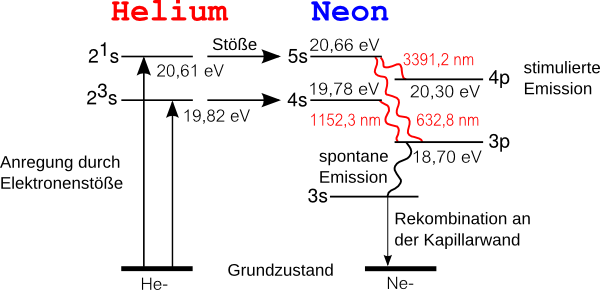
\includegraphics[width=\textwidth]{content/HeNe-Laser_Energieüberträge.png}
  \caption{Schematische Darstellung der Energieübergänge zwischen den Atomen im Resonator eines HeNe-Lasers bei äußerer Anregung \cite{HeNe_Übergänge}.}
  \label{fig:HeNe-Laser_Energieüberträge}
\end{figure}

\subsection{Der Resonator}
Der Resonator in dem sich das aktive Medium befindet ist durch zwei Spiegel begrenzt. Einer dieser Spiegel ist voll reflektierend und der andere, der Auskoppelspiegel, reflektiert so viele Photonen, dass die Gesamtverluste während eines
Durchlaufs des Resonators durch neu erzeugte Photonen ausgeglichen werden. Die ausgekoppelten Photonen verlassen den Resonator und bilden den Strahl. Damit dieser Prozess im Resonator stabil ablaufen kann, muss der Resonator die
Stabilitätsbedingung \ref{eqn:Stabilitätsbedingung} erfüllen,
\begin{equation}
	0 < g_1 g_2 < 1
\label{eqn:Stabilitätsbedingung}
\end{equation}
hierbei sind $g_1$ und $g_2$ die Stabilitätsfaktoren der Spiegel. Diese können über \ref{eqn:Stabilitätsfaktoren} aus der Länge des Resonators $L$ und dem Krümmungsradius des jeweiligen Spiegels $R_i$ bestimmt werden.
\begin{equation}
	g_i = 1 - \frac{L}{R_i}
\label{eqn:Stabilitätsfaktoren}
\end{equation}
Die im Laser erzeugten Photonen haben eine, gegen die Länge des Resonators $L$, sehr kleine Wellenlänge $\lambda$. Durch die wiederholten Reflexionen an den Spiegeln bildet sich im Resonator eine stabile Feldverteilung aus. Hierbei kann
zwischen der Feldverteilung entlang und senkrecht zur Resonatorachse unterschieden werden. Für die Ausbildung der transversalen Moden des Resonators ist die Verteilung senkrecht zur Resonatorachse verantwortlich. Diese möglichen transversalen 
Feldverteilungen werden als TEM-Moden bezeichnet. Sie unterscheiden sich in der räumlichen Intensitätsverteilung senkrecht zum Laserstrahl. Hierbei kann die Intensitätsverteilung der $TEM_{00}$ Mode durch die 
Gaußverteilung \ref{eqn:Intensität00} 
\begin{equation}
	I_{00}(x, y) = I_0 \exp{\left(\frac{-2(x^2+y^2)}{\omega^2}\right)}
\label{eqn:Intensität00}
\end{equation}
beschrieben werden und die der $TEM_{10}$ Mode durch \ref{eqn:Intensität10}, wobei $\omega$ der Strahlradius ist.
\begin{equation}
	I_{10}(x, y) = I_0 \frac{8x^2}{\omega^2} \exp{\left(\frac{-2(x^2+y^2)}{\omega^2}\right)}
\label{eqn:Intensität10}
\end{equation}
Hierbei sind die Vorfaktoren der e-Funktionen die Produkte der Quadrate der Hermite-Polynome $H_n(z)$ mit $z = \frac{\sqrt{2}x_{1/2}}{\omega}$. Der Index $n$ ist hierbei je einer der Indizes der Intensität $I_{ij}$. Allgemein kann die
Intensität $I_{ij}$ über \ref{eqn:Intensitätij} bestimmt werden.
\begin{equation}
	I_{ij}(x, y) = I_0 \left(H_i^2\left(\frac{\sqrt{2}x}{\omega}\right) \cdot H_j^2\left(\frac{\sqrt{2}y}{\omega}\right)\right) \exp{-\frac{2(x^2+y^2)}{\omega^2}}
\label{eqn:Intensitätij}
\end{equation}
Die longitudinalen Moden beschreiben die Feldverteilung entlang der Resonatorachse. Diese unterscheiden sich in der Frequenz. Damit sich eine longitudinale Resonatormode ausbilden kann, muss das Lichtfeld nach einem vollständigen Umlauf
im Resonator wieder dieselbe Phase besitzen. Hieraus ergibt sich die Resonanzbedingung \ref{eqn:Resonanzbedingung_Longitudinal} mit der Resonatorlänge $L$, der Wellenlänge der q-ten Mode $\lambda_q$ und der Modenzahl $q$.
\begin{equation}
	\lambda_q = \frac{2L}{q}
	\label{eqn:Resonanzbedingung_Longitudinal}
\end{equation}
Dies führt zu einem Frequenzabstand $\Delta f$ der über \ref{eqn:Frequenzabstand} berechnet werden kann, wobei $c$ die Lichtgeschwindigkeit ist.
\begin{equation}
	\Delta f = \frac{c}{2L}
	\label{eqn:Frequenzabstand}
\end{equation}



\subsection{Bewegung der Atome im Gas}
Die Atome in einem Gas befinden sich bei Temperaturen über dem absoluten Nullpunkt nie in Ruhe. Die mikroskopische Bewegung der Atome wird durch die makroskopische Temperatur $T$ beschrieben. Die Bewegung der Atome führt bei Emission eines 
Photons dazu, dass dieses Photon im Laborsystem nicht exakt die Wellenlänge des Übergangs der es erzeugt hat, sondern um die Bewegung des Atoms verschoben ist. Dieser Effekt wird als Dopplereffekt bezeichnet. Die Größe des Frequenzbereichs
$\Delta f_D$ kann bei bekannter Temperatur $T$ und bekannter erwarteter Frequenz aus dem Übergang $f_0$ über $\ref{eqn:Frequenz_Doppler}$ bestimmt werden. Dabei ist $k_B$ die Boltzmann Konstante $c$ die Lichtgeschwindigkeit und $m$ die Masse
der betrachteten Atome. Die im Falle des HeNe-Lasers relevanten Atome sind die Neonatome. 
\begin{equation}
	\Delta f_D = f_0 \sqrt{\frac{8k_BT\ln(2)}{mc^2}}
	\label{eqn:Frequenz_Doppler}
\end{equation}





\pagebreak
